\section{Dettagli matematici e numerici delle campagne E1 e F1}
\label{app:stageef}\label{app:solver_supplement}

\subsection{Numero di Péclet direzionale}

Per la mesh ALE si considera la velocità relativa $\boldsymbol\beta=\bm b-\bm w$ e, per ogni elemento $K$,
\begin{equation}
Pe_K=\frac{\norm{\boldsymbol\beta}h_K^\beta}{2\nu},\qquad
h_K^\beta=\frac{2\norm{\boldsymbol\beta}}{\sum_i|\boldsymbol\beta\cdot\nabla\varphi_i|}.
\label{eq:peclet_local}
\end{equation}
Per velocità relativa nulla si pone $Pe_K=0$. Sulla mesh fissa, $Pe_K=7.8125$; per ALE, al tempo $t=0.25$, mediana, 95-esimo percentile e massimo sono rispettivamente 8.91, 10.84 e 11.11.


\subsection{Confronto Galerkin/SUPG e work--precision}

La SUPG è stata confrontata con Galerkin su mesh $32\times32$ e $\Delta t=0.0025$. Nella configurazione fissa l'errore $L^2$ assoluto medio passa da $4.262\times10^{-3}$ a $4.302\times10^{-3}$; nel test ALE mobile, basato su una deformazione armonica prescritta e indipendente da GDM, passa da $4.597\times10^{-3}$ a $4.653\times10^{-3}$. Non emerge un miglioramento di accuratezza nella configurazione esaminata. La deformazione armonica non è una prova di convergenza ALE mobile.


Il work--precision a $\Delta t=0.0025$ usa un warm-up escluso e cinque ripetizioni di timing: gli errori medi sono $1.074\times10^{-2}$, $4.262\times10^{-3}$ e $3.048\times10^{-3}$ per $16^2$, $32^2$ e $64^2$; i tempi mediani sono 0.059, 0.200 e 0.735 s. La curva è operativa a passo fisso e non isola completamente l'errore spaziale a $64^2$.

\begin{figure*}[!t]
\centering
\begin{minipage}[t]{0.32\textwidth}
\centering
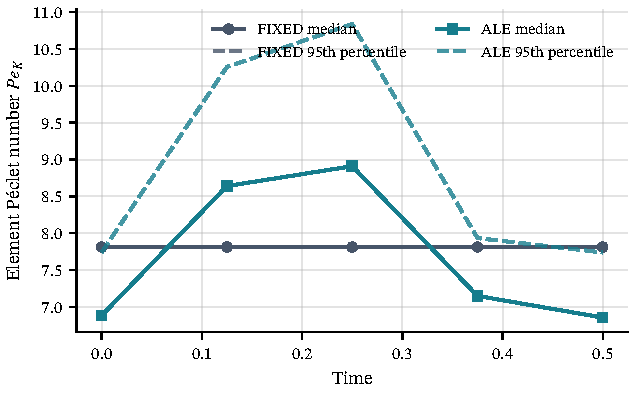
\includegraphics[width=\linewidth,height=0.14\textheight,keepaspectratio]{images/stage_e/peclet_distribution.pdf}
\captionof{figure}{Péclet direzionale su mesh fissa e ALE.}
\label{fig:app_peclet}
\end{minipage}\hfill
\begin{minipage}[t]{0.32\textwidth}
\centering
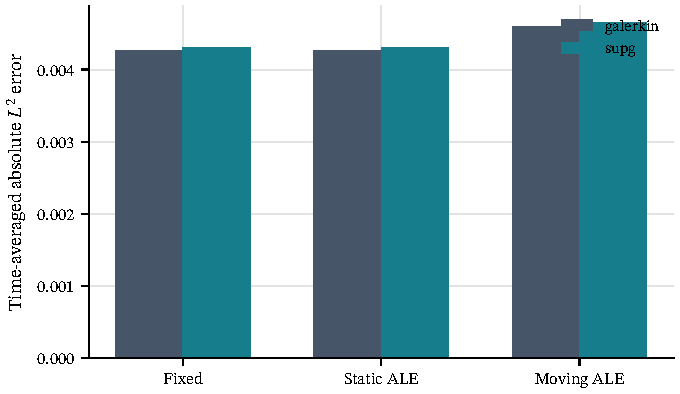
\includegraphics[width=\linewidth,height=0.14\textheight,keepaspectratio]{images/stage_e/supg_comparison.pdf}
\captionof{figure}{Confronto Galerkin/SUPG nella configurazione E1.}
\label{fig:app_supg}
\end{minipage}\hfill
\begin{minipage}[t]{0.32\textwidth}
\centering
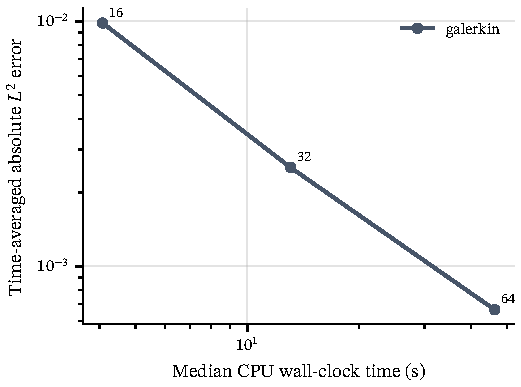
\includegraphics[width=\linewidth,height=0.14\textheight,keepaspectratio]{images/stage_e/work_precision_galerkin_temporally_resolved.pdf}
\captionof{figure}{Work--precision Galerkin su mesh fisse.}
\label{fig:app_workprecision}
\end{minipage}
\end{figure*}



\subsection{Lemma di esattezza del punto medio per la D-GCL}

\begin{lemma}[Esattezza geometrica nel singolo passo]
Sia $K(t)$ un triangolo affine $P_1$ in due dimensioni, i cui nodi seguono traiettorie lineari nel tempo su $[t_n,t_{n+1}]$. Si assuma che il Jacobiano orientato resti positivo nell'intero intervallo, che la velocità nodale sia costante a tratti e che i contributi geometrici siano integrati con quadratura spaziale esatta di grado almeno due. Allora la regola del punto medio integra esattamente, nel singolo passo, la derivata temporale della matrice di massa geometrica associata all'elemento.
\label{lem:dgcl_midpoint}
\end{lemma}

\begin{proof}
La mappa isoparametrica $F_K(\hat{\bm x},t)$ è affine rispetto alle coordinate di riferimento e lineare in $t$. Il gradiente $J_K(t)=\nabla_{\hat{\bm x}}F_K(t)$ è quindi una matrice $2\times2$ affine nel tempo. Il determinante $\det J_K(t)$ è un polinomio in $t$ di grado al più due; di conseguenza la sua derivata è affine. La regola del punto medio è esatta per polinomi di grado non superiore a uno e integra quindi esattamente la variazione del determinante nel passo. Poiché le funzioni di forma $P_1$ sono fisse nella coordinata di riferimento, la matrice di massa geometrica è il prodotto tra integrali di forma e determinante Jacobiano. La quadratura spaziale esatta e l'identità precedente implicano l'esattezza dell'incremento geometrico della matrice di massa.
\end{proof}

Il lemma riguarda l'identità geometrica discreta sotto le ipotesi indicate. Non implica stabilità, convergenza del solver ALE, conservazione della massa della PDE forzata o positività in aritmetica floating-point.

\subsection{Monitor MMPDE e selezione su validation}

I monitor classici sono costruiti dal campo FEM corrente:
\begin{align}
G_{\mathrm{arc}}&=I+\alpha\nabla u_h\nabla u_h^T,\\
G_{\mathrm{W}}&=\sqrt{\det(G_{\mathrm{arc}})}\,I,\\
G_{\mathrm{H}}&=I+\alpha|H_h|.
\end{align}
L'Hessiano è ricostruito ai nodi mediante least-squares pesato sui patch a due anelli, poiché l'Hessiano elementare di un campo $P_1$ è nullo all'interno di ciascun elemento. I monitor sono simmetrizzati, proiettati su matrici definite positive e smussati; l'evoluzione pseudo-temporale usa gradienti discreti, precondizionamento mass-lumped, bordo vincolato e line-search. Il budget è 200 iterazioni per evento. Sono stati raggiunti i limiti in 19/280 eventi Winslow, 2/280 arc-length e 5/280 Hessian-based; questo non equivale a convergenza certificata.

\begin{table*}[!t]
\centering\small
\caption{Griglia discreta di selezione dell'intensità dei monitor sulla validation ($n=12$). I valori sono quelli valutati, non una ricerca continua.}
\label{tab:f1_alpha_validation}
\begin{tabular*}{\textwidth}{@{\extracolsep{\fill}}lrrrr}
\toprule
Monitor & $\alpha$ & Errore medio $L^2$ [\%] & Eventi al cap /120 & Esito\\
\midrule
Winslow & 0.0100 & 8.1201 & 0 & \\
Winslow & 0.0250 & 8.0854 & 1 & \\
Winslow & 0.0500 & 8.0509 & 0 & \\
Winslow & 0.1000 & 8.0098 & 5 & Selezionato\\
\midrule
Arc-length & 0.0100 & 8.0939 & 0 & \\
Arc-length & 0.0250 & 8.0566 & 0 & Selezionato\\
Arc-length & 0.0500 & 8.0934 & 0 & \\
Arc-length & 0.1000 & 8.4114 & 4 & \\
\midrule
Hessian & 0.0001 & 8.1491 & 0 & \\
Hessian & 0.0005 & 8.1476 & 0 & \\
Hessian & 0.0010 & 8.1434 & 0 & \\
Hessian & 0.0050 & 8.1290 & 1 & Selezionato\\
\bottomrule
\end{tabular*}
\end{table*}

\subsection{Risposta descrittiva al parametro \texorpdfstring{$\sigma$}{sigma}}

I 28 casi F1 sono ordinati per $\sigma$ e suddivisi in quattro gruppi consecutivi di sette casi. La tabella riporta riduzioni medie appaiate; si tratta di statistiche descrittive post hoc, non di una legge causale. Il parametro $\beta$ varia simultaneamente.
\begin{table}[!t]
\centering\scriptsize
\caption{Riduzione relativa media dell'errore integrato di GDM nei gruppi ordinati per $\sigma$ del test F1.}
\label{tab:f1_sigma_groups}
\resizebox{\columnwidth}{!}{%
\begin{tabular}{@{}llrrrr@{}}
\toprule
Gruppo & Intervallo $\sigma$ & Fixed [\%] & Winslow [\%] & Arc-length [\%] & Hessian [\%]\\
\midrule
Q1 & [0.02236, 0.03037] & 6.80 & 3.41 & 6.15 & 5.97\\
Q2 & [0.03115, 0.05436] & 7.28 & 5.34 & 6.73 & 6.75\\
Q3 & [0.05764, 0.08794] & 8.73 & 7.31 & 7.35 & 8.68\\
Q4 & [0.08887, 0.10339] & 9.34 & 8.33 & 7.69 & 9.82\\
\bottomrule
\end{tabular}%
}
\end{table}

\subsection{Definizioni del tracking e del filtro}

La corona diagnostica è definita da $0.5\sigma\le r\le2\sigma$ rispetto al centro gaussiano mobile. Indicando con $\mathcal K(t)$ l'insieme degli elementi e con $\mathcal K_A(t)$ quelli il cui baricentro ricade nella corona $A_\sigma(t)$, l'arricchimento di densità è
\begin{equation}
E_\rho(t)=\frac{|\mathcal K_A(t)|/|\mathcal K(t)|}{|A_\sigma(t)|/|\Omega|}.
\label{eq:annular_enrichment}
\end{equation}
Il denominatore normalizza la frazione di elementi rispetto alla sola frazione di area occupata dalla corona, intersecata con il dominio. Un valore maggiore di uno indica una concentrazione di elementi nella regione, non necessariamente una riduzione uniforme della dimensione degli elementi. Il rapporto $R_h=\bar h_\Omega/\bar h_A$ confronta le scale caratteristiche globali e locali; analogamente, $R_h>1$ è coerente con elementi mediamente più piccoli nella corona. La distanza tra il centro gaussiano e il centroide diagnostico della concentrazione è espressa in unità di $\sigma$. Queste quantità sono state calcolate su quattro traiettorie validation, con 404 snapshot complessivi, e non costituiscono statistiche held-out.

Nel campione osservato, l'arricchimento mediano è $1.213$ e il rapporto mediano $R_h$ è $1.111$. La distanza normalizzata centroide--sorgente ha mediana $0.49\sigma$ sull'intera sequenza e $0.61\sigma$ agli istanti finali. Le misure documentano una risposta locale della risoluzione alla regione mobile, ma anche un inseguimento non esatto: l'arricchimento è moderato e la distanza non si annulla. La lettura va inoltre distinta dal requisito, non necessario per una mesh $r$-adattiva, di collocare un vertice esattamente nel massimo del campo. La diagnostica valuta la distribuzione degli elementi intorno alla regione localizzata, non la coincidenza tra un nodo e il picco della soluzione.

Il filtro applica un fattore globale $\alpha\in[0,1]$ al segmento tra mesh corrente e proposta raw,
\begin{equation}
\bm X(\alpha)=\bm X^n+\alpha\,\Delta\bm X_{\mathrm{raw}},\qquad
J_K(\alpha)=A_K\alpha^2+B_K\alpha+C_K.
\label{eq:filter_path_polynomial}
\end{equation}
Per elementi affini $P_1$, il determinante orientato è quadratico lungo il segmento. Il fattore accettato è limitato dal primo vincolo di ammissibilità incontrato considerando tutti gli elementi, con la convenzione di blocco dei nodi di bordo. Si tratta di un limitatore globale della lunghezza del passo: una singola cella può quindi ridurre lo spostamento di tutti i nodi interni, anche quando la cella limitante è lontana dalla regione di interesse.

Nelle 40 finestre diagnostiche validation il filtro interviene in 32 eventi ($80\%$); la mediana di $\alpha$ è $0.423$, il quinto percentile è $3.29\times10^{-6}$ e il rapporto mediano tra norma dello spostamento accettato e proposta raw è $0.481$. Le proposte raw contengono elementi invertiti in 16 eventi, mentre non se ne osservano dopo il filtro. Questi dati mostrano che il filtro modifica in modo sostanziale una parte delle proposte, ma non dimostrano che ogni intervento sia causato da un'inversione già presente: il vincolo agisce lungo l'intero percorso. Il minimo Jacobiano post-filtro registrato, $9.999999999999865\times10^{-5}$ per $\epsilon=10^{-4}$, differisce dalla soglia di circa $1.35\times10^{-18}$. La discrepanza è compatibile con l'arrotondamento in doppia precisione e impedisce di interpretare il filtro come garanzia stretta in aritmetica floating-point.
